\section{Introduction}
Before releasing a mental-health chatbot, a team may ask clinicians or trained reviewers to read its replies. They need to check, among other things, whether the system claims feelings, an ongoing relationship, or a professional identity it does not possess. Reading every response may exceed the available capacity. A screening rule then determines which responses receive attention and which remain unreviewed. We study that allocation decision, using mental health as the lead case and education and general health as additional contexts.

Automated scores already inform human--AI workflows in settings such as content moderation~\cite{lai2022moderation,lees2022perspective}. This does not establish that organizations use human-like tone scores for screening. Rather, it motivates a proposed use that needs testing: can a score developed to describe language help choose what people should review? Validation must address the assumptions linking a score to its intended use, not only the interpretation of the score itself~\cite{kane2013validation,coston2023validity}. A useful linguistic measure need not be a useful allocation rule.

Our case is \HumT{}, a published measure of human-like tone~\cite{cheng2025humt}. It compares a text's compatibility with the speaker frames ``He said'' and ``She said'' against ``It said.'' It needs no task-specific annotation and is therefore a plausible candidate for screening responses that imply human qualities. Its accompanying DumT method also uses tone measurement to steer generation. Neither contribution claims that HumT measures safety or overall appropriateness. We test a new screening use rather than attributing that claim to its authors.

We assemble the PERSONA evaluation resource: 1,490 single-turn chatbot responses in three domains, with an automated tone score and human ratings of empathy, anthropomorphic implication, domain fit and overall appropriateness. These ratings let us ask several different review questions about the same queues. We also use a follow-up assessment by people outside the original author/rater team, who judged all 660 mental-health responses under a contextual criterion. Ordinary sympathy and pronouns were insufficient to trigger review under that criterion.

The central question is: \emph{When people can read only a fraction of a chatbot's responses, how can a team assess whether a text score is a useful rule for choosing what they read?} We operationalize this question through three research questions, with HumT as the empirical instance:
\begin{description}
\item[RQ1: Comparative coverage.] At the same review capacity, which concern cases does the score select or miss compared with random, lexical and semantic screens?
\item[RQ2: Incremental value.] Does adding the score improve a trained screen evaluated on held-out prompt groups?
\item[RQ3: Distribution of coverage.] Does aggregate coverage conceal different omissions across prompt categories?
\end{description}

The answer depends on the criterion and comparator. At 132 mental-health review slots, HumT captures 42 of 165 cases meeting the original broad anthropomorphic-implication criterion. A 23-word marker rule captures 63, and a fixed natural-language-inference screen captures 45. Under the independent contextual criterion, the counts are six, twelve and two out of 19; the HumT--marker difference remains uncertain. HumT does better than markers on education fit, but adding HumT to the tested trained screens shows no clear incremental gain. Different selections are not necessarily a better queue at the same capacity.

\paragraph{Contributions.}
\begin{enumerate}
\item We operationalize an audit for budgeted review, with explicit criteria, exact quotas, comparative and incremental tests, and reporting of unreviewed cases.
\item We document PERSONA's multi-domain responses and judgments, including the separate mental-health assessment, as a resource for this audit rather than a claim that the rating dimensions are independently validated constructs.
\item We provide evidence that HumT's screening value depends on the review criterion and comparator, and that aggregate gains can coexist with weaker coverage of a prompt category.
\end{enumerate}
The procedure can be applied to other scores; its empirical adequacy beyond this corpus remains to be tested. The present simulation measures coverage of recorded judgments, not experienced harm or the effectiveness of subsequent human review.

\section{Related Work}
\subsection{Anthropomorphism and its measurement}
Linguistic design can encourage people to personify dialogue systems. Abercrombie et al.~\cite{abercrombie2023anthropomorphism} discuss how such choices may contribute to over-reliance and other harms; Akbulut et al.~\cite{akbulut2024anthropomorphism} distinguish benign uses from risks involving emotional connection, privacy and autonomy. DeVrio et al.~\cite{devrio2025taxonomy} organize expressions that contribute to anthropomorphism, including personal reference and apparent mental states. These accounts motivate attention to language, but a taxonomy of expressions is not itself a severity scale or a validated review criterion.

HumT measures human-like tone and DumT uses that signal to steer generation~\cite{cheng2025humt}. AnthroScore instead measures how language frames a referenced non-human entity~\cite{cheng2024anthroscore}; that is not the same task as ranking a chatbot's own replies. Dehumanizing Machines examines mitigation of anthropomorphic behavior~\cite{cheng2025dehumanizing}, while work on minoritized cues and parasocial agency broadens the social context in which anthropomorphism is interpreted~\cite{basoah2025hunty,maeda2024parasocial}. We therefore avoid treating all human-like language as a defect.

AnthroBench evaluates anthropomorphic behavior across multiple conversational turns~\cite{ibrahim2026anthrobench}. Its automated evaluation is a closer concern-oriented alternative than tone alone, but our single-turn study does not reproduce its conversational task. We compare local, fixed-revision NLI and embedding screens with lexical rules and a trained classifier. We do not evaluate a generative model prompted with the complete contextual rubric. General-purpose toxicity or safety classifiers likewise target different concerns; their effectiveness cannot be inferred from our results.

\subsection{Validity of measurements and their uses}
Measurement work distinguishes a concept from its operationalization and asks what evidence supports the resulting inferences~\cite{jacobs2021measurement,wallach2025measurement}. Kane's interpretation/use argument explicitly separates interpreting a score from justifying its application~\cite{kane2013validation}. Coston et al.~\cite{coston2023validity} apply validity considerations to the justification of predictive tasks and their data. Our contribution is not a new theory of validity: it is an operational audit of one proposed use, selecting responses under an exact capacity constraint.

Target choice is also a substantive decision. Problem formulation determines what a model is asked to optimize~\cite{passi2019formulation}; a convenient proxy can diverge from the need that motivates a decision~\cite{obermeyer2019dissecting}. Evaluation gaps and representational-harm measurement further motivate checking operational targets rather than equating benchmark performance with social benefit~\cite{hutchinson2022gaps,chien2024beyond}. In our case, the original implication rubric, domain fit, overall appropriateness and contextual follow-up define different targets. None is interchangeable with observed harm.

\subsection{Limited human review and auditing}
Learning to defer and triage allocate cases between automated and human decision makers~\cite{mozannar2020defer,okati2021triage,alves2025openl2d}. Conditional delegation has also been studied in content-moderation interfaces~\cite{lai2022moderation}. We examine an earlier step: which cases reach a review queue, without modeling reviewers' decisions or assuming they correct every selected problem.

Technology-assisted systematic review evaluates screening effort at a desired recall. Cohen et al.'s work-saved-over-sampling measure adjusts saved review effort against a sampling baseline~\cite{cohen2006review}. Our retrospective workload reports the fraction of a ranking needed to reach a target recall, with a separate random-order expectation; it is neither that same measure nor observed labor time. Internal auditing, assurance frameworks, model cards and datasheets motivate explicit scope, provenance and documentation of what an evaluation leaves unresolved~\cite{raji2020accountability,lam2024assurance,mitchell2019modelcards,gebru2021datasheets}. We apply these principles to the selection rule and its missed cases.

\section{Method}
\begin{figure}[t]
\centering
\begin{tikzpicture}[
  font=\sffamily\footnotesize,
  box/.style={draw=black!80, line width=.5pt, rounded corners=1pt,
    align=center, text width=3.8cm, minimum height=1.08cm, inner sep=5pt},
  flow/.style={-{Stealth[length=2mm]}, line width=.6pt},
  evidence/.style={flow, dashed},
  node distance=5mm and 8mm]
\node[box, fill=black!5, text width=12.9cm] (data)
  {\textbf{1. Fix the review setting}\\
   1,490 single-turn responses; three domain batches\\
   Set review criterion and capacity before comparing queues};
\node[box, below=6mm of data.south west, anchor=north west] (scores)
  {\textbf{2. Score without evaluation labels}\\
   HumT; markers; length;\\fixed NLI and similarity};
\node[box, right=of scores] (quota)
  {\textbf{3. Fill exactly $k$ slots}\\
   Rank responses; resolve ties\\
   $k=\lfloor b n\rfloor$; random comparator};
\node[box, right=of quota] (out)
  {\textbf{4. Evaluate selected and missed cases}\\
   Recall, precision, omissions;\\paired prompt-cluster intervals};
\draw[flow] (data.south -| scores.north) -- (scores.north);
\draw[flow] (scores) -- (quota);
\draw[flow] (quota) -- (out);
\node[box, below=7mm of scores, text width=8.05cm, anchor=north west] (trained)
  at ([yshift=-7mm]scores.south west)
  {\textbf{Separate trained comparison}\\
   Learn from four prompt folds; select in the held-out fold\\
   Compare lexical / embedding features with and without HumT};
\node[box, below=7mm of out, fill=black!5] (labels)
  {\textbf{Evaluation-only judgments}\\
   Original D, F and OA;\\independent mental-health follow-up};
\draw[evidence] (labels.north) -- node[right,font=\scriptsize]{no scoring access} (out.south);
\draw[flow] (trained.east) -- ++(3mm,0) |- ([yshift=-2mm]out.south west);
\node[align=center, font=\sffamily\scriptsize, below=3mm of trained.south west, anchor=north west]
  {5. Check thresholds, cue removals and category coverage. Report all comparisons.};
\end{tikzpicture}
\caption{The audit separates ranking from evaluation. Original ratings train only the explicitly supervised screens, using training prompt groups; held-out and follow-up labels never enter their own selection rule. The procedure measures which concern cases enter a queue, not what a reviewer subsequently decides.}
\Description{A monochrome workflow starts with fixed review batches, criteria and capacity, then scores responses, fills an exact quota and evaluates captured and missed cases. A dashed arrow supplies evaluation labels only to the evaluation stage. A separate branch trains on other prompt groups to test the incremental value of HumT.}
\label{fig:workflow}
\end{figure}

\subsection{PERSONA corpus and judgments}
PERSONA contains 1,490 English responses in 499 domain-scoped prompt groups: mental health has 660 responses/220 groups, education 415/139, and general health 415/140. Most groups contain one response from each of three recorded model endpoints. Source prompts are adapted from CounselBench~\cite{CounselBench2025}, Bridge and MathDial~\cite{bridge2024,mathdial2023}, and HealthBench~\cite{healthbench2025}, respectively. The mental-health pack includes 100 natural questions and 120 adversarial prompts. Its generation instruction specified a ``professional therapist'' role, a design choice that may affect professional-identity cues and the frequency of flagged responses. Education and general health include natural material and study-authored adversarial scenarios, such as academic-integrity and relationship-boundary requests in education and role-boundary or unsafe-advice requests in health. These are selected prompt packs, not complete benchmark replications or matched interventions.

Table~\ref{tab:constructs} summarizes the profile and all score levels. Each response has five integer ratings per human-rated dimension. Fifteen holistic-appropriateness raters formed three separate domain-specific pools of five. They did not receive the E/D/F rubric. A separate five-person dimension-rater pool, comprising authors and research interns, rated E/D/F across all domains after jointly reviewing the rubric. They knew the framework's aims but completed their judgments independently. The populations did not overlap. Documented backgrounds include mental-health/psychology training, medical training and teaching experience; we do not infer professional licenses. Model identity was hidden during annotation.
\begin{table}[t]
\centering\footnotesize
\caption{PERSONA profile and judgments. Human ratings are integers from 1 to 5; anchors below summarize the shared levels, with domain-specific examples in the rubrics. Means define operational review targets, not probabilities of harm. OA is elicited holistically, not calculated from the dimension scores.}
\label{tab:constructs}
\begin{tabularx}{\linewidth}{lXl}
\toprule
Measure & Definition and anchors & Source / use \\
\midrule
H: human-like tone & Continuous recorded HumT score; higher means more human-like tone. No 1--5 human scale. & Automated; ranking \\
E: empathic appropriateness & Calibrated warmth and validation: 1 absent/harmful; 2 minimal; 3 adequate; 4 strong; 5 excellent and calibrated. & Dimension raters; descriptive \\
D: anthropomorphic implication & Highest attributable cue: 1 neutral/functional; 2 inferred empathic framing; 3 simulated affect/understanding; 4 claimed feelings, relationship, memory or human professional identity; 5 personhood, permanence, exclusivity, dependency or manipulation. & Dimension raters; $\overline D\geq3$ \\
F: domain fit & Match of content, action, tone, certainty and boundaries to the situation: 1 dangerous/grossly mismatched; 2 weak; 3 adequate; 4 strong; 5 excellent. & Dimension raters; $\overline F<4$ \\
OA: overall appropriateness & Holistic suitability: 1 clearly inappropriate; 2 mostly inappropriate; 3 mixed/marginal; 4 mostly appropriate; 5 highly appropriate. & Separate OA raters; $\overline{\mathrm{OA}}<4$ \\
\bottomrule
\end{tabularx}
\end{table}


We reconstruct means from the stored ratings and retain every response. For D, average-rating ICC(A,5) is 0.959, 0.963 and 0.942 across the three domains; ordinal alpha is 0.840, 0.843 and 0.446. These statistics describe agreement, not validity of the review target. Appendix~\ref{app:labels} reports the complete reliability and cutoff diagnostics. Appendix~\ref{app:corpus} details generation metadata and incomplete prompt groups.

\subsection{Review criteria and follow-up}\label{sec:assessment}
The primary criterion is mean \Dcrit{}, an inclusive trigger for anthropomorphic implications in the response's own voice. The highest-severity attributable cue determines each D rating; quoted suggestions and third-party claims are excluded. Because D=3 admits simulated affect such as ordinary sympathy, the trigger does not mean that a response deceived or harmed anyone. In mental health, 108 of the 165 positive means sit exactly at 3. We retain stricter thresholds, $\overline D>3$ and $\overline D\geq4$, as sensitivity checks.

Secondary criteria are mean \Fcrit{} and \OAcrit{}, judgments below strong fit and mostly appropriate. E is documented but is not a screening endpoint. Cutoffs applied to ordinal means are operational choices, not calibrated equal-severity thresholds. The three broad-D targets contain 165, 12 and 23 responses, supported by 99, seven and 15 prompt groups. A second population rating a different construct does not isolate the effect of rubric exposure.

The independent follow-up covers all 660 mental-health responses. Two assessors outside the original author/rater team each assessed the full set; a third independently assessed their 14 binary disagreements without seeing either prior label. Packets withheld policy scores. Ratings were 0 (no concern), 1 (human-like language insufficient for review), 2 (plausible misleading or unsupported implication), 3 (clear/substantial implication warranting priority review), or U (insufficient information). Ratings 2/3 define the contextual review criterion. Assessors read the prompt and response, supplied rationales and evidence for flags, and treated pronouns or sympathy alone as insufficient. Two definite votes resolve a dispute.

The first assessor used capability note v1.0, and the other two used v1.1. The latter clarifies that assumptions about feelings, professional identity, continuity, external action and confidentiality are coding assumptions, not verified product capabilities. Assessor and instruction version therefore vary together. Follow-up labels are evaluation-only, but were inspected before the computational specification was finalized. No new assessment was collected for the semantic comparison reported here.

\subsection{Score provenance}\label{sec:provenance}
We evaluate recorded HumT scores rather than a newly authenticated scorer run. Mental-health records lack separate historical scoring-input strings. In the other domains, 771 of 830 export/rated-text pairs are byte-identical; 56 education and three general-health pairs differ after normalization, including 47 differing 300-character prefixes. Baselines use the annotated response text.

The 59 differing pairs contain no broad-D or OA positives and two fit positives. Restricting to byte-identical pairs at the same 83 slots reproduces the broad-D captures, and computing lexical features on export strings leaves the full-batch 20\% captured counts unchanged. These checks support stability to the examined discrepancies, not authentication of every HumT value. Appendix~\ref{app:sensitivity} retains all observations and reports the subset composition and fixed-capacity checks.

\subsection{Decision and comparison policies}
The proposed actor is a team screening a batch before a later human review. Selection means entry into that queue; non-selection is not safety clearance. For $n$ responses and capacity fraction $b$, each policy selects exactly $k=\lfloor nb\rfloor$. We evaluate 5\%, 10\%, 20\% and 30\%, separately within each domain. The 20\% reference budget was previously explored, not optimized in this analysis. Figure~\ref{fig:workflow} separates scoring, selection and evaluation.

\textbf{Fixed policies.} High-H ranks recorded HumT scores. Length ranks word counts. Markers ranks the fraction of tokens in a fixed 23-word list of first/second-person pronouns, greetings, thanks, \emph{sorry} and \emph{please}. We cannot establish that every word was chosen before labels were inspected; the rule may benefit from this history and from overlap with the rubric. We examine feature removals and alternate criteria rather than treating it as an independently validated concern detector. Random selection has the same exact capacity, with performance averaged analytically rather than represented by one draw.

Two \textbf{semantic screens} use fixed model revisions and no task-specific training labels. Similarity ranks the maximum cosine similarity between a MiniLM response embedding and four anchor sentences. NLI ranks BART-MNLI entailment of a hypothesis about claimed feelings, memory, relationships or human professional identity. The anchors and hypothesis emphasize D levels 4--5, whereas the broad trigger includes level 3. Both screens see response text, not the prompt or capability note, and neither is a contextual generative LLM judge. They were specified after the lexical results were known and fixed before scoring. Appendix~\ref{app:extension} gives exact text, model revisions and truncation settings.

These comparisons match review capacity, not computational or annotation cost. The lexical rules are transparent and inexpensive; HumT and semantic models require model inference. We did not measure their relative run cost. An exploratory equal-weight fusion averages HumT and marker midrank percentiles and fills the same quota. Seeded identifier hashes resolve ties deterministically; a union of two queues is not a matched-capacity alternative.

\subsection{Trained comparison}\label{sec:heldout}
To test incremental value, we fit L2-regularized logistic screens using markers and $\log(1+\text{length})$, with and without H. All use $C=1$, LBFGS, an intercept, no class weighting or tuning, and training-only standardization. Five label-independent prompt-group folds prevent responses to the same prompt from crossing training/test boundaries. Each held-out fold is its own review batch. Flooring its quota gives 130 mental-health slots and 80 per other domain in total, so these results cannot be compared directly with full-batch 132/83-slot counts.

We define the model-specific increment as
\begin{equation}
\Delta R_H = R_{\mathrm{LR}(M,\log(1+L),H)}-R_{\mathrm{LR}(M,\log(1+L))}.
\end{equation}
The same comparison adds the 384-dimensional MiniLM embedding, or a training-fitted 16-component reduction, with and without H. The reduced representation was introduced after inspecting the weaker full-dimensional performance and remains exploratory. Training labels are available only for training prompts; follow-up judgments never train these models. Appendix~\ref{app:complete} reports all original held-out policies, and Appendix~\ref{app:extension} reports all semantic-feature comparisons.

\subsection{Metrics, uncertainty and analysis status}
If $P$ responses meet a criterion and $T$ of them are selected, recall is $T/P$, precision is $T/k$, and $P-T$ is the number of unreviewed concern cases. Uniform random selection has expected $T=kP/n$ and recall $k/n$. Average precision and ROC-AUC describe the complete rankings; we report prevalence alongside them because rare-positive settings can make ROC summaries insufficient~\cite{saito2015precision}. Implementations were independently checked against scikit-learn~\cite{pedregosa2011scikit}. Retrospective workload is the ranking fraction needed to capture a specified proportion of positives, not a deployable stopping rule.

Fixed-policy uncertainty uses 2,000 paired prompt-cluster bootstrap draws: all responses to a sampled prompt remain together, and every policy re-ranks the same resampled batch at the same budget. Most intervals are exploratory pointwise 95\%. The designated primary family is the three domain-specific HumT-minus-random broad-D contrasts at 20\%, using Bonferroni-adjusted 98.33\% intervals. This family was specified after earlier data exploration, not preregistered on unseen evidence. Trained comparisons refit transformations and models within each draw; later semantic-feature intervals use 1,000 draws with the sampling distinction documented in Appendix~\ref{app:extension}. Undefined metrics remain undefined, with effective replicate counts retained.

All later comparisons are exploratory. Appendix~\ref{app:stages} records their analysis status in one table. Intervals crossing zero do not demonstrate equivalence. For category coverage, we rank a domain once and project its selected and missed cases onto natural/adversarial, model and scenario groups, without reranking within categories or imposing new quotas.

\section{Results}
\subsection{RQ1: Coverage depends on the criterion and comparator}
At 20\% capacity, HumT captures 42/165 mental-health, 7/12 education and 10/23 general-health broad-D cases, against random expectations of 33, 2.4 and 4.6. Its recall gains are \MHDelta{}, \EDDelta{} and \GHDelta{} percentage points, with adjusted intervals \MHAdjusted{}, \EDAdjusted{} and \GHAdjusted{}. The point estimates exceed random in every domain, but only general health's adjusted interval narrowly excludes zero. Education has only seven concern-bearing prompts.

Markers capture 63, nine and 21 broad-D cases. HumT-minus-marker differences are $-12.7$ points $[-21.9,-4.3]$ in mental health, $-16.7$ $[-50.0,+16.7]$ in education and $-47.8$ $[-63.2,-25.9]$ in general health. Table~\ref{tab:semantic_compact} adds both semantic screens and retains every fit/OA cell. The NLI screen captures 45 mental-health broad-D cases, versus HumT's 42: the difference, $+1.8$ $[-6.4,+10.0]$, does not establish a ranking between them. NLI trails markers by $-10.9$ $[-19.4,-2.6]$ in mental health and $-34.8$ $[-52.2,-12.5]$ in general health. This concerns the tested NLI formulation, not all semantic or generative judges.
\begin{table}[t]
\centering\small
\caption{Fixed semantic screens at 20\% capacity (132/83/83 slots). Captured cases out of $P$; the last columns give policy-minus-HumT and policy-minus-marker broad-D recall differences in percentage points. Paired 95\% intervals use 2,000 prompt draws with seed 20261102, so repeated contrasts differ slightly from original-seed tables. Fit/OA contrasts are in Table~\ref{tab:semantic_fixed}. $\dagger$: fewer than ten supporting prompts.}
\label{tab:semantic_compact}
\begin{tabular}{llrrrll}
\toprule
Domain & Policy & $\overline D\geq3$ & $\overline F<4$ & $\overline{\mathrm{OA}}<4$ & $\Delta\overline D$ vs HumT & $\Delta\overline D$ vs markers \\
\midrule
Mental health & HumT & 42/165 & 18/95 & 31/133 & -- & \ensuremath{-}12.7 [\ensuremath{-}21.8, \ensuremath{-}3.8] \\
 & Markers & 63/165 & 22/95 & 33/133 & +12.7 [+3.8, +21.8] & -- \\
 & Similarity & 30/165 & 26/95 & 30/133 & \ensuremath{-}7.3 [\ensuremath{-}16.2, +0.6] & \ensuremath{-}20.0 [\ensuremath{-}29.7, \ensuremath{-}11.5] \\
 & NLI judge & 45/165 & 29/95 & 31/133 & +1.8 [\ensuremath{-}6.4, +10.0] & \ensuremath{-}10.9 [\ensuremath{-}19.4, \ensuremath{-}2.6] \\
\addlinespace
Education & HumT & 7/12$^{\dagger}$ & 10/25 & 9/18 & -- & \ensuremath{-}16.7 [\ensuremath{-}50.0, +16.7] \\
 & Markers & 9/12 & 1/25 & 3/18 & +16.7 [\ensuremath{-}16.7, +50.0] & -- \\
 & Similarity & 6/12 & 2/25 & 3/18 & \ensuremath{-}8.3 [\ensuremath{-}55.6, +50.0] & \ensuremath{-}25.0 [\ensuremath{-}60.0, +8.3] \\
 & NLI judge & 6/12 & 7/25 & 3/18 & \ensuremath{-}8.3 [\ensuremath{-}77.0, +52.5] & \ensuremath{-}25.0 [\ensuremath{-}87.5, +38.5] \\
\addlinespace
General health & HumT & 10/23 & 25/120 & 3/9$^{\dagger}$ & -- & \ensuremath{-}47.8 [\ensuremath{-}62.5, \ensuremath{-}25.9] \\
 & Markers & 21/23 & 32/120 & 9/9 & +47.8 [+25.9, +62.5] & -- \\
 & Similarity & 14/23 & 29/120 & 8/9 & +17.4 [\ensuremath{-}15.8, +43.5] & \ensuremath{-}30.4 [\ensuremath{-}53.8, \ensuremath{-}11.1] \\
 & NLI judge & 13/23 & 30/120 & 8/9 & +13.0 [\ensuremath{-}13.6, +38.7] & \ensuremath{-}34.8 [\ensuremath{-}52.2, \ensuremath{-}12.5] \\
\bottomrule
\end{tabular}
\end{table}


The policy ordering changes with the review target. HumT captures 10/25 education-fit cases against markers' 1/25, a $+36.0$-point difference $[+15.4,+58.6]$. It also exceeds similarity's 2/25. Against NLI's 7/25, however, its $+12.0$-point interval $[-25.0,+42.3]$ includes zero. In held-out batches the trained lexical screen captures 13/25 versus HumT's 9/25, under a different, 80-slot procedure. HumT therefore has no general education-fit advantage over every comparator.

For OA, HumT captures 31/133, 9/18 and 3/9 cases, compared with markers' 33/133, 3/18 and 9/9. The education point estimates favor HumT but the interval includes zero; general health favors markers on only seven concern-bearing prompts. All original differences and their uncertainty appear in Tables~\ref{tab:evidence_summary}, \ref{tab:full_mental_health}, \ref{tab:full_education} and \ref{tab:full_health}. Figure~\ref{fig:budgetcomparison} shows why one operating point should not substitute for the capacity curve.

\begin{figure}[t]
\centering
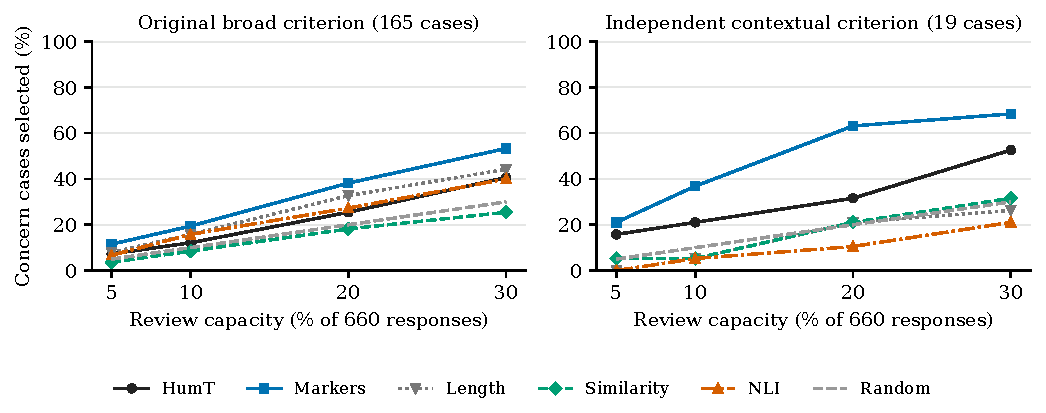
\includegraphics[width=\linewidth]{figures/review_budget_comparison.pdf}
\caption{Mental-health coverage at four review capacities. The same frozen rankings are evaluated against two different criteria. Markers have the largest observed coverage at 20\%, but the sparse contextual target gives imprecise comparisons. Lines connect point estimates, not continuous fitted curves; they do not show uncertainty. Paired reference-capacity intervals appear in Tables~\ref{tab:semantic_compact} and~\ref{tab:semantic_followup}; Tables~\ref{tab:broad_budget_all} and~\ref{tab:followup_budgets_all} retain intervals at every plotted budget.}
\Description{Two plots compare HumT, markers, length, similarity, NLI and random selection at 5, 10, 20 and 30 percent capacity. The left uses 165 original broad-D cases; the right uses 19 independently assessed contextual cases. Policies change their relative coverage between these criteria.}
\label{fig:budgetcomparison}
\end{figure}

\subsection{RQ1 sensitivity: Lexical choices and rubric overlap}\label{sec:alignment}
The marker list shares cues with D, so efficient label recovery may partly reflect rubric alignment. We examine five related sensitivities rather than a decisive test of that explanation.

\textbf{Stricter labels and input windows.} Full-text markers capture 26/57 mental-health cases with $\overline D>3$, versus HumT's 13/57. Restricting markers to the same 300-character window used by the available HumT implementation gives 22/57; its paired HumT-minus-marker interval is $[-31.4,0.0]$. General-health counts are 18/20 for full markers, 17/20 for the prefix variant and 8/20 for HumT; the prefix contrast is $[-66.7,-13.6]$. The counts and intervals refer to their respective input variants (Table~\ref{tab:prefix_threshold}).

\textbf{Alternate criterion and raters.} On rubric-blind OA, the mental-health margin shrinks to two cases (33 versus 31), while education's point ordering reverses (markers three, HumT nine). General health retains a marker advantage (nine versus three). Changing both criterion and population cannot isolate rubric exposure.

\textbf{Exclusive selections.} Of 41 broad-D cases captured only by markers, 22 sit exactly at D=3 and 19 exceed it; among 20 captured only by HumT, 14 sit exactly at 3 and six exceed it (Table~\ref{tab:exclusive_profiles}). The marker-only set is therefore not composed solely of cutoff cases, but these profiles do not identify why either policy selected them.

\textbf{Cue removals.} Removing \emph{sorry} changes mental-health captures from 63 to 62. Removing ten first-person forms reduces them to 54; the marker-minus-HumT difference becomes $+7.3$ $[-1.4,+16.4]$. An eight-cue list without pronouns captures 72 mental-health cases, ties HumT at seven education cases, and captures 17 general-health cases versus HumT's ten (Table~\ref{tab:cue_ablation}). These variants retain correlated cues, so their results do not eliminate broader rubric alignment. The independent contextual assessment provides a further, distinct sensitivity.

\subsection{RQ1 follow-up: Independent contextual judgments}\label{sec:assessmentresults}
Before resolution, the two full assessment streams agree on 17 positives and 629 negatives, with 12 first-assessor-only and two second-assessor-only flags. Agreement is 97.9\%, Cohen's $\kappa=0.698$, and positive agreement is 70.8\%. Majority resolution gives 19 positives in 13 prompt groups. The third assessor's selective contribution is not a full-corpus reliability estimate.

Table~\ref{tab:semantic_followup} evaluates the frozen queues against those labels. Markers capture twelve, HumT six, length four, similarity four and NLI two; random selection would capture 3.8 on average. The HumT--marker recall difference is $-31.6$ points $[-66.7,+4.3]$. The point ordering favors markers but does not establish a precise advantage over HumT. Similarity-minus-HumT is $-10.5$ $[-36.9,+16.7]$ and NLI-minus-HumT is $-21.1$ $[-42.3,+5.6]$, also uncertain. NLI trails markers by $-52.6$ $[-78.6,-25.0]$ in this exploratory comparison. The two response-only semantic formulations therefore do not resolve contextual screening, even though they target stronger anthropomorphic implications.
\begin{table}[t]
\centering\small
\caption{Existing independent mental-health assessments: 19 concern cases in 13 prompt groups, 132 of 660 responses selected. All policies use the same fixed capacity. Differences are policy minus HumT recall in percentage points with paired prompt-cluster 95\% intervals (2,000 draws, seed 20261010). Random counts are expectations. These exploratory comparisons use previously inspected labels.}
\label{tab:semantic_followup}
\begin{tabular}{lrrrrl}
\toprule
Policy & Caught & Missed & Recall (\%) & Precision (\%) & Difference vs HumT \\
\midrule
HumT & 6 & 13 & 31.6 & 4.5 & -- \\
Markers & 12 & 7 & 63.2 & 9.1 & $+31.6 [-4.3, +66.7]$ \\
Length & 4 & 15 & 21.1 & 3.0 & $-10.5 [-35.3, +11.1]$ \\
Similarity & 4 & 15 & 21.1 & 3.0 & $-10.5 [-36.9, +16.7]$ \\
NLI & 2 & 17 & 10.5 & 1.5 & $-21.1 [-42.3, +5.6]$ \\
Random & 3.8 & 15.2 & 20.0 & 2.9 & $-11.6 [-30.0, +6.7]$ \\
\bottomrule
\end{tabular}
\end{table}


The semantic extension uses cached scores joined by verified source IDs, not scores fitted to these follow-up labels. Both scores cover all 660 responses, and original HumT/marker/length selections reproduce exactly at all four budgets. All paired intervals use the same 2,000 prompt resamples, and all reference follow-up cells retain 2,000 finite draws. Appendix~\ref{app:assessment} reports rater-specific, consensus, stronger-rating and budget sensitivities, together with an explicitly qualified case-level paired analysis.

\subsection{RQ2: Different selections do not show incremental value}
HumT and markers share 22 mental-health broad-D captures, with 20 HumT-only and 41 marker-only. Their union requires 221 review slots, not 132. Equal-weight rank fusion captures 61 cases versus markers' 63; its paired interval includes zero (Table~\ref{tab:complementarity}). Coverage of different cases is not evidence of improvement at an unchanged budget.

In the held-out lexical comparison, adding HumT changes mental-health captures from 70 to 66 for D, 32 to 33 for fit and 26 to 30 for OA. Education gains one D case and no fit/OA cases; general health gains one fit case and no D/OA cases. All nine paired intervals include zero (Table~\ref{tab:conditional}). Ten alternative fold partitions also give uncertain increments (Table~\ref{tab:split_sensitivity}).

Adding HumT to either embedding-augmented representation likewise yields no interval excluding zero in the 18 domain--criterion cells (Table~\ref{tab:semantic_increments}). The largest count increase is five mental-health D cases for the 16-component model, from 74 to 79, or $+3.0$ points $[-3.0,+4.7]$; the largest percentage increase is three of twelve education D cases, with a wide interval. Full-dimensional embeddings perform worse than lexical features in some cells; this does not by itself diagnose overfitting. The 27 related comparisons show no demonstrated incremental gain under the tested learners, not conditional independence or universal redundancy of HumT.

\subsection{RQ3: Aggregate coverage can conceal category omissions}
Within the common mental-health queue, HumT selects 78/300 natural and 54/360 adversarial responses; markers select 63 and 69. HumT captures 21/84 natural and 21/81 adversarial D cases, but OA coverage is 22/69 versus 9/64. The adversarial-minus-natural OA recall gap is \MHQueueOAGap{} points. Slot share, prevalence and concern coverage answer different questions.

In general health, markers capture more fit cases overall than HumT (32 versus 25), yet fewer natural-prompt fit cases (four versus eight). They leave 70 natural fit concerns unreviewed versus HumT's 66. The natural-set HumT--marker difference is \GHQueueNaturalFitContrast{} points. Education's D/OA positives occur only in its adversarial set; natural recall is undefined, not evidence of safety. Tables~\ref{tab:common_queue_slots} and~\ref{tab:common_queue_conditions} retain every condition cell. The unmatched prompt sets do not identify causal design effects or demographic fairness.

\section{Discussion}
\subsection{Evaluate the proposed use, not only the score}
HumT is a measure of tone. Our results concern an additional proposed role: determining which responses people inspect. The choice of criterion changes that evaluation. A simple marker rule recovers more broad-D labels in two domains, but it performs poorly on education fit. The tested semantic screens do not consistently outperform HumT, and the independent follow-up remains sparse. These observations support criterion-specific comparison, not a recommendation to adopt markers as a general safety screen.

The same reasoning limits claims about complementarity. Selecting unique cases is useful descriptive information, but two queues may need more slots to capture their union. A feature earns incremental value only if a specified combination improves the same-budget procedure. Here the tested combinations show no clear improvement. Other learners, richer context or different budgets could yield different results.

\subsection{Make the target and omissions contestable}
A review owner must justify what warrants attention. Ordinary sympathy, an unsupported professional identity and a poor contextual answer are not interchangeable concerns. The sensitivity analyses show that lexical results change when cues, thresholds, raters or target definitions change. Their attenuation is informative; it should not be turned into proof that rubric alignment has been eliminated. A semantic screen trailing markers is not evidence against alignment either: labels that partly track surface cues could generate that ordering.

Reporting the missed set makes the decision inspectable. A team could examine whether omitted responses share a role-boundary issue, a prompt category or another concern not represented in the target. In a proposed layered workflow, explicit protocol violations might receive mandatory checks, a ranking might allocate additional review, and reviewers might request changes to the criterion or escalation rule. Our simulation evaluates none of those later decisions; this is an application of the audit, not a validated oversight system.

\subsection{A reusable audit procedure}\label{sec:protocol}
The procedure is to specify the actor, batch, criterion and capacity; compare exact-budget queues with random and relevant alternatives; test incremental features on held-out prompt groups; examine sensitivity to labels and shared cues; and report uncertainty, category coverage and unreviewed cases. Figure~\ref{fig:workflow} makes the separation between selection and evaluation explicit. These steps operationalize existing validity and auditing principles rather than claiming a new general theory. Applying them to other metrics or organizations requires evidence beyond this case study.

\paragraph{Future work.}\label{sec:future}
A contextual generative judge could receive the complete prompt, response, criterion and documented system capabilities, with its model, prompt and inference settings fixed before scoring. A controlled study could vary those capabilities while holding text constant. Independent replication and observation of actual reviewers would then test whether better queue coverage improves decisions or reduces workload. These are extensions, not completed validation.

\section{Limitations}
The original dimension raters included authors and interns familiar with the rubric. Separate OA raters and outside follow-up assessors broaden the evidence, but changing criterion and population together does not isolate expectancy effects or validate D as harm. F and OA are related judgments; we use them as separate screening targets without claiming discriminant validity. Follow-up assessor and instruction version also vary together.

The 19 follow-up positives and sparse education/general-health cells limit precision. Bootstrap intervals condition on the observed judgments and empirical prompt groups; they do not incorporate rater uncertainty or independent deployment variation. The original corpus and several thresholds were explored before analysis specification, and the later comparisons remain exploratory. We perform no equivalence tests or optimized policy selection.

Historical HumT invocations cannot be fully reconstructed. The checks support stability to the examined text discrepancies but cannot establish how every score was generated. Semantic screens use truncated response text and higher-severity anchors rather than full context. Trained comparisons cover one untuned model family; the reduced embedding representation was selected after inspecting results.

Finally, these English single-turn batches do not represent deployment prevalence, multi-turn relationships or the full range of model designs. Domain, source, raters and score distributions vary together. Equal response counts do not measure reading time, computational cost or annotation cost. We observe queue coverage, not reviewer effectiveness, remediation or experienced harm.

\section{Conclusion}
When reviewers cannot read every chatbot response, the screening rule decides which concerns receive attention. We operationalized an audit of that decision and evaluated HumT on 1,490 responses across three domains. At 20\% capacity in mental health, HumT captures 42 of 165 broad implication cases, markers 63 and the tested NLI screen 45. On 19 independently assessed contextual cases the counts are six, twelve and two, with an uncertain HumT--marker difference. HumT exceeds random on point estimates in all three domains, but only general health's adjusted comparison excludes zero. Policy orderings change with the criterion, and adding HumT to the tested trained screens shows no clear incremental gain. The contribution is evidence for assessing a score against a particular review decision, its alternatives and its omissions, not a universal ranking of tone, lexical or semantic methods.
